\documentclass[12pt,a4paper]{article}

\usepackage[utf8]{inputenc}
\usepackage[T1]{fontenc}
\usepackage[spanish,es-nodecimaldot]{babel}
\usepackage{geometry}
\usepackage{setspace}
\usepackage{graphicx}
\usepackage{booktabs}
\usepackage{tabularx}
\usepackage{longtable}
\usepackage{array}
\usepackage{multirow}
\usepackage{float}
\usepackage{amsmath,amssymb}
\usepackage{caption}
\usepackage{subcaption}
\usepackage{xcolor}
\usepackage{enumitem}
\usepackage{fancyhdr}
\usepackage{listings}
\usepackage[hidelinks]{hyperref}
\usepackage[nameinlink,noabbrev]{cleveref}

\geometry{margin=2.5cm}
\setstretch{1.15}
\setlength{\parskip}{0.4em}
\setlength{\parindent}{0pt}

\hypersetup{
		colorlinks=true,
		linkcolor=blue,
		urlcolor=blue,
		citecolor=blue
}

\lstdefinestyle{pythoncompact}{
	language=Python,
	basicstyle=\ttfamily\scriptsize,
	keywordstyle=\color{blue},
	stringstyle=\color{green!60!black},
	commentstyle=\color{gray},
	showstringspaces=false,
	breaklines=true,
	breakatwhitespace=false,
	columns=fullflexible,
	keepspaces=true,
	tabsize=4,
	frame=single,
	xleftmargin=0.8em,
	xrightmargin=0.3em,
	postbreak=\mbox{\textcolor{gray}{$\hookrightarrow$}\space}
}

\lstset{
		style=pythoncompact
}

\setlength{\parskip}{0.6em}
\setlength{\parindent}{0pt}
\onehalfspacing

\pagestyle{fancy}
\fancyhf{}
\fancyhead[L]{Tarea de minería de datos y modelización predictiva}
\fancyhead[R]{\thepage}

% ---------- PORTADA ----------
\newcommand{\universidad}{UNIVERSIDAD COMPLUTENSE DE MADRID}
\newcommand{\facultad}{Facultad de Estudios Estadísticos}
\newcommand{\grado}{Máster en Big Data, Data Science \& Inteligencia Artificial}
\newcommand{\curso}{2025--2026}
\newcommand{\ciudad}{Madrid}

\newcommand{\titulo}{Clasificación binaria de churn con selección de variables y redes neuronales}
\newcommand{\autor}{Daniel Olmedo Rawlins Poveda}
\newcommand{\asignatura}{Tarea de minería de datos y modelización predictiva}
\newcommand{\profesor}{Pablo Arcadio Flores}
\newcommand{\fecha}{\today}

\begin{document}

\begin{titlepage}
	\centering
	\vspace*{0.5cm}

	\begin{minipage}{0.45\textwidth}
		\centering
		\IfFileExists{figures/ucm-logo.png}{%
			\includegraphics[width=3.4cm]{figures/ucm-logo.png}%
		}{%
			\vspace*{3.4cm}%
		}
	\end{minipage}%
	\begin{minipage}{0.45\textwidth}
		\centering
		\IfFileExists{figures/ntic-master.png}{%
			\includegraphics[width=4.6cm]{figures/ntic-master.png}%
		}{%
			\vspace*{3.4cm}%
		}
	\end{minipage}

	\vspace{0.5cm}

	{\Large \textbf{\universidad}}\\[0.25cm]
	{\large \facultad}\\[0.1cm]
	{\large \grado}

	\vfill

	{\LARGE \textbf{\titulo}}\\[0.5cm]
	{\large \textit{Tarea de} \asignatura}

	\vfill

	\begin{flushleft}
	\setlength{\tabcolsep}{6pt}
	\renewcommand{\arraystretch}{1.2}
	\begin{tabular}{@{}ll}
		\textbf{Autor:} & \autor \\
		\textbf{Profesor:} & \profesor \\
		\textbf{Curso académico:} & \curso \\
	\end{tabular}
	\end{flushleft}

	\vfill

	{\ciudad, \fecha}
\end{titlepage}

\clearpage
\pagenumbering{roman}

\begin{abstract}
Este documento presenta el desarrollo completo de una tarea de clasificación binaria sobre churn. Se analizan los datos, se depuran y se evalúan dos flujos principales: uno orientado a maximizar Accuracy mediante RFE con regresión logística y una red neuronal, y otro orientado a maximizar Recall a partir de variables relevantes obtenidas con un árbol de decisión y una red neuronal posterior.
\end{abstract}

\tableofcontents
\newpage

\pagenumbering{arabic}

\section{Introducción}

En esta sección se presenta el objetivo del trabajo, el contexto del problema de churn y la estructura general del informe. También se adelantan los criterios metodológicos que guían el análisis, el preprocesamiento, la selección de variables y la comparación entre modelos.

\subsection{Objetivo}

Describir el problema, justificar el enfoque experimental y situar el resto de apartados dentro de un protocolo reproducible.

\section{Descripción del conjunto de datos}

El conjunto de datos utilizado en este trabajo corresponde a clientes de una empresa de telecomunicaciones y tiene como finalidad predecir el riesgo de abandono del servicio. La base está formada por veinte variables explicativas, denotadas como \(V1\) a \(V20\), y una variable objetivo \(Y\), que identifica si el cliente ha abandonado o no la compañía.

Desde un punto de vista conceptual, las variables disponibles recogen distintas dimensiones del comportamiento del cliente, incluyendo información territorial, características del contrato, uso del servicio y relación con la empresa. Esta estructura sugiere la posible existencia de variables identificadoras, variables categóricas codificadas numéricamente y relaciones de dependencia entre variables de uso y facturación.

\subsection{Variables y objetivo}

La variable objetivo del problema es \(Y\), que toma valor \(1\) cuando el cliente abandona el servicio y valor \(0\) en caso contrario, configurando así un problema de clasificación binaria.

Las variables explicativas pueden agruparse en distintas categorías:

\begin{itemize}
    \item \textbf{Identificación y localización}: \(V1\) (estado o región), \(V3\) (código de área) y \(V4\) (número de teléfono). Estas variables pueden incluir información categórica o identificadora, siendo especialmente relevante el carácter no predictivo esperado de \(V4\).
    
    \item \textbf{Características del cliente}: \(V2\) (duración de la cuenta), que refleja la antigüedad del cliente en la compañía.
    
    \item \textbf{Servicios contratados}: \(V5\) (plan internacional), \(V6\) (plan de buzón de voz) y \(V7\) (número de mensajes), que capturan el tipo de servicios activos.
    
    \item \textbf{Uso y facturación}: \(V8\)–\(V19\), que recogen minutos, número de llamadas y costes asociados en distintos periodos (diurno, vespertino, nocturno e internacional). Estas variables presentan potenciales relaciones de dependencia, ya que los costes suelen derivarse directamente del uso.
    
    \item \textbf{Atención al cliente}: \(V20\) (número de llamadas al servicio de atención), que puede actuar como indicador de insatisfacción o problemas con el servicio.
\end{itemize}

Esta clasificación inicial permite anticipar distintos tratamientos en la fase de preprocesamiento, especialmente en lo relativo a la codificación de variables categóricas, la eliminación de identificadores y la detección de posibles redundancias.
\section{Análisis y depuración de datos}

En esta sección se recopilan los resultados del control de calidad de los datos, la gestión de valores perdidos, el tratamiento de posibles anomalías, la detección de redundancias y las transformaciones aplicadas antes del modelado.

\subsection{Criterios de depuración}

Se detallarán aquí las decisiones adoptadas y su justificación metodológica.

\subsection{Feature engineering}

Se describirán las transformaciones adicionales realizadas para mejorar la capacidad predictiva o la estabilidad de los modelos.

\section{Protocolo experimental}

En esta sección se define el protocolo común para todos los experimentos, con el objetivo de garantizar comparabilidad entre enfoques y evitar \textit{data leakage}. El protocolo se aplica sobre el conjunto de modelado resultante de la Fase 1 \((3538, 16)\).

\subsection{Partición y validación}

Se adopta un esquema en dos niveles:

\begin{enumerate}
	\item \textbf{Partición externa estratificada}: separación inicial en \textit{train\_val} y \textit{test} mediante una única semilla fija (\texttt{random\_state = 42}). El conjunto de test queda bloqueado para evaluación final.
	\item \textbf{Validación interna estratificada}: dentro de \textit{train\_val}, uso de validación cruzada estratificada para seleccionar variables, hiperparámetros y umbral.
\end{enumerate}

Reglas operativas comunes:

\begin{itemize}
	\item Imputación, codificación y escalado se ajustan exclusivamente con datos de entrenamiento en cada pliegue.
	\item Cualquier selección de variables (RFE o importancia del árbol) se realiza dentro del marco de validación.
	\item El conjunto de test no interviene en la elección de transformaciones, hiperparámetros ni umbral.
\end{itemize}

\subsection{Validación de candidatas de feature engineering}

Las variables candidatas propuestas tras el EDA (tabla \texttt{fase2\_feature\_candidates.csv}) no se incorporan de forma automática. Su adopción se decide con una regla explícita de validación para evitar sobreajuste por diseño.

Para cada candidata (o bloque coherente de candidatas), se comparan dos configuraciones en validación cruzada sobre \textit{train\_val}:

\begin{itemize}
	\item \textbf{Modelo base}: sin la nueva transformación.
	\item \textbf{Modelo extendido}: incluyendo la transformación candidata.
\end{itemize}

El criterio de aceptación será:

\begin{enumerate}
	\item \textbf{Apartado orientado a Accuracy}: aceptar la candidata solo si mejora la Accuracy media de validación y no produce una caída relevante de Recall (caída absoluta mayor de 0.02).
	\item \textbf{Apartado orientado a Recall}: aceptar la candidata solo si mejora la Recall media de validación y no provoca un deterioro severo de Precision o PR-AUC (caída absoluta mayor de 0.02 en ambos indicadores).
	\item \textbf{Estabilidad}: en ambos apartados, la desviación estándar entre pliegues no debe aumentar de forma marcada respecto al modelo base (incremento superior al 20\% como señal de inestabilidad).
\end{enumerate}

Adicionalmente, si dos transformaciones ofrecen mejoras similares, se priorizará la alternativa más interpretable y con menor complejidad del pipeline.

\subsection{Selección de umbral}

La selección de umbral se realiza exclusivamente con predicciones de validación interna. Se evalúa una rejilla de umbrales y se guarda una tabla de métricas por umbral.

\begin{itemize}
	\item En el bloque de Accuracy, se selecciona el umbral que maximiza Accuracy manteniendo degradación de Recall controlada.
	\item En el bloque de Recall, se selecciona el umbral que prioriza captación de churn y se reporta explícitamente el coste en falsos positivos.
\end{itemize}

El umbral final elegido en validación se aplica una única vez sobre test.

\subsection{Métricas}

Las métricas comunes para todos los experimentos son:

\begin{itemize}
	\item Accuracy,
	\item Recall,
	\item Precision,
	\item F1-score,
	\item ROC-AUC,
	\item PR-AUC,
	\item matriz de confusión.
\end{itemize}

La métrica primaria cambia según el objetivo del apartado (Accuracy en el modelo 1 y Recall en el modelo 2), pero la interpretación final se realiza siempre de forma multivariable para evitar conclusiones sesgadas por un único indicador.

\section{Modelo orientado a Accuracy}

El diseño inicial de esta fase se basó en una cadena \textit{RFE + MLP}: primero se realizó selección de variables con RFE (estimador lineal) y, sobre ese subconjunto, se entrenó una red neuronal multicapa optimizada con validación cruzada estratificada. Como paso posterior, y manteniendo el mismo protocolo experimental, se evaluaron modelos alternativos de ensamble para intentar mejorar la métrica objetivo (\textit{Accuracy}).

El criterio de selección se mantuvo constante durante toda la fase: elección por rendimiento en validación interna y evaluación final en el conjunto de test bloqueado, sin recalibrar umbrales con información de test.

\subsection{Selección de variables con RFE}

Sobre la representación preprocesada del bloque lineal se aplicó RFE con regresión logística, fijando $k=5$ variables. El subconjunto seleccionado en esta etapa fue:

\begin{itemize}
	\item \texttt{nominal\_\_V1\_4.0}
	\item \texttt{nominal\_\_V1\_24.0}
	\item \texttt{nominal\_\_V1\_31.0}
	\item \texttt{numeric\_\_V20}
	\item \texttt{numeric\_\_V8}
\end{itemize}

Este bloque produjo un modelo base competitivo y permitió establecer una referencia inicial para Accuracy en test.

\subsection{Ajuste del modelo y selección final}

En una primera iteración se optimizó una MLP con \texttt{GridSearchCV} sobre arquitectura, activación, regularización y tasa de aprendizaje. Esa variante obtuvo un rendimiento de referencia de aproximadamente \textbf{0.8559} en Accuracy sobre test.

Dado que existía margen de mejora, se ejecutó una segunda iteración de búsqueda sobre modelos de ensamble de árboles (Random Forest y Extra Trees), manteniendo validación cruzada estratificada y selección de umbral en validación interna. El mejor candidato por validación cruzada fue \textbf{Random Forest}, adoptado como modelo final de Accuracy.

\begin{table}[h]
\centering
\caption{Resultados finales del modelo orientado a Accuracy (test)}
\begin{tabular}{|l|c|}
\hline
Modelo final & \texttt{RF\_Accuracy} \\
\hline
Umbral de decisión & 0.49 \\
\hline
Accuracy & 0.9492 \\
\hline
Recall & 0.8156 \\
\hline
Precision & 0.9200 \\
\hline
F1-score & 0.8647 \\
\hline
ROC-AUC & 0.9211 \\
\hline
PR-AUC & 0.8968 \\
\hline
Matriz de confusión $(TN,FP,FN,TP)$ & $(557,10,26,115)$ \\
\hline
\end{tabular}
\end{table}

La mejora respecto al baseline MLP fue sustancial: $0.9492 - 0.8559 = 0.0933$ puntos absolutos de Accuracy. Este resultado confirma que, para el objetivo de calidad global de clasificación, el ensamble de árboles captura mejor la estructura no lineal del problema en comparación con el modelo neuronal inicial.

\section{Árbol de decisión y red neuronal optimizada en Recall}

En esta sección se entrena un árbol de decisión para identificar variables relevantes y se construye una red neuronal posterior optimizada para Recall con búsqueda paramétrica exhaustiva.

\subsection{Importancia de variables}

Se detallará el criterio seguido para seleccionar las variables más relevantes a partir del árbol.

\subsection{Ajuste de la red neuronal}

Se presentarán los hiperparámetros evaluados, el umbral seleccionado y la evaluación completa del modelo.

\section{Comparación global}

Esta sección resume la comparación final entre ambos enfoques, manteniendo foco en rendimiento en test, sensibilidad al umbral e implicaciones operativas.

\subsection{Desempeño predictivo en test}

Ambos modelos se evaluaron con el mismo protocolo (split externo 75/25 y validación cruzada estratificada 5-fold). La selección de umbral se realizó en validación interna y el contraste final en test.

\subsubsection{Métricas finales}

\begin{table}[h]
\centering
\small
\begin{tabular}{lccccccc}
\toprule
\textbf{Modelo} & \textbf{Umbral} & \textbf{Accuracy} & \textbf{Recall} & \textbf{Precisión} & \textbf{F1} & \textbf{ROC-AUC} & \textbf{PR-AUC} \\
\midrule
ET\_Recall  & 0.14 & 0.548 & 0.943 & 0.299 & 0.454 & 0.927 & 0.881 \\
RF\_Accuracy & 0.49 & 0.949 & 0.816 & 0.920 & 0.865 & 0.921 & 0.897 \\
\bottomrule
\end{tabular}
\caption{Desempeño final en el conjunto de test. ET: Extra Trees. RF: Random Forest.}
\label{tab:final_performance}
\end{table}

\begin{figure}[h]
\centering
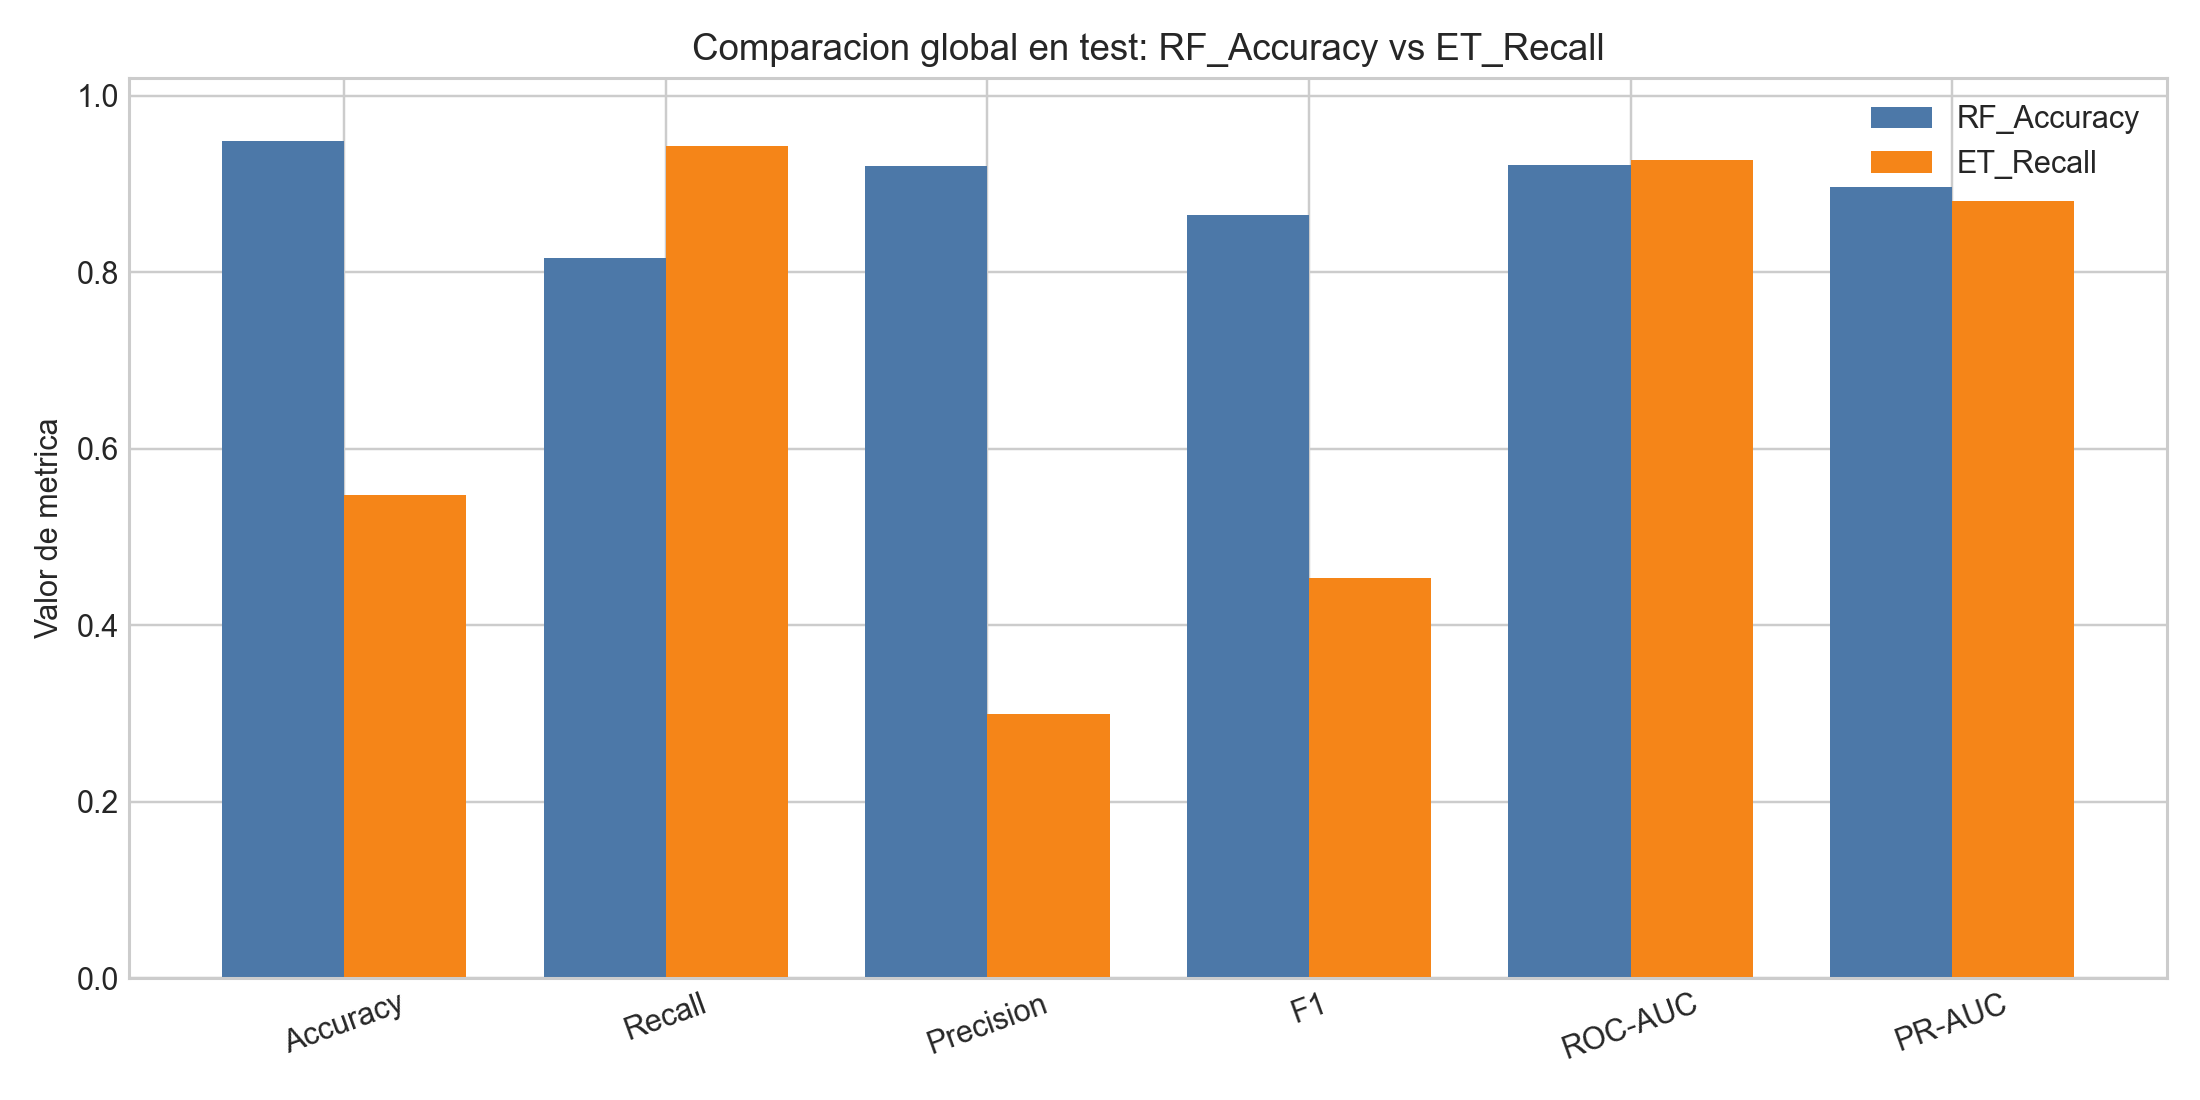
\includegraphics[width=0.92\textwidth]{figures/fase3_model_comparison_bars.png}
\caption{Comparación visual de métricas en test para RF\_Accuracy y ET\_Recall.}
\label{fig:comparacion_global_barras}
\end{figure}

RF\_Accuracy ofrece mejor desempeño global (Accuracy y Precision altas), mientras que ET\_Recall maximiza la cobertura de churn a costa de más falsos positivos.

\subsection{Trade-off entre objetivos}

El análisis del espacio de threshold confirma un intercambio claro entre cobertura y precisión:

\begin{itemize}
  \item \textbf{RF\_Accuracy}: su mejor compromiso se alcanza en threshold 0.49.
  \item \textbf{ET\_Recall}: mantiene recall alto con menor threshold, pero incrementa de forma notable los falsos positivos.
\end{itemize}

\begin{figure}[h]
\centering
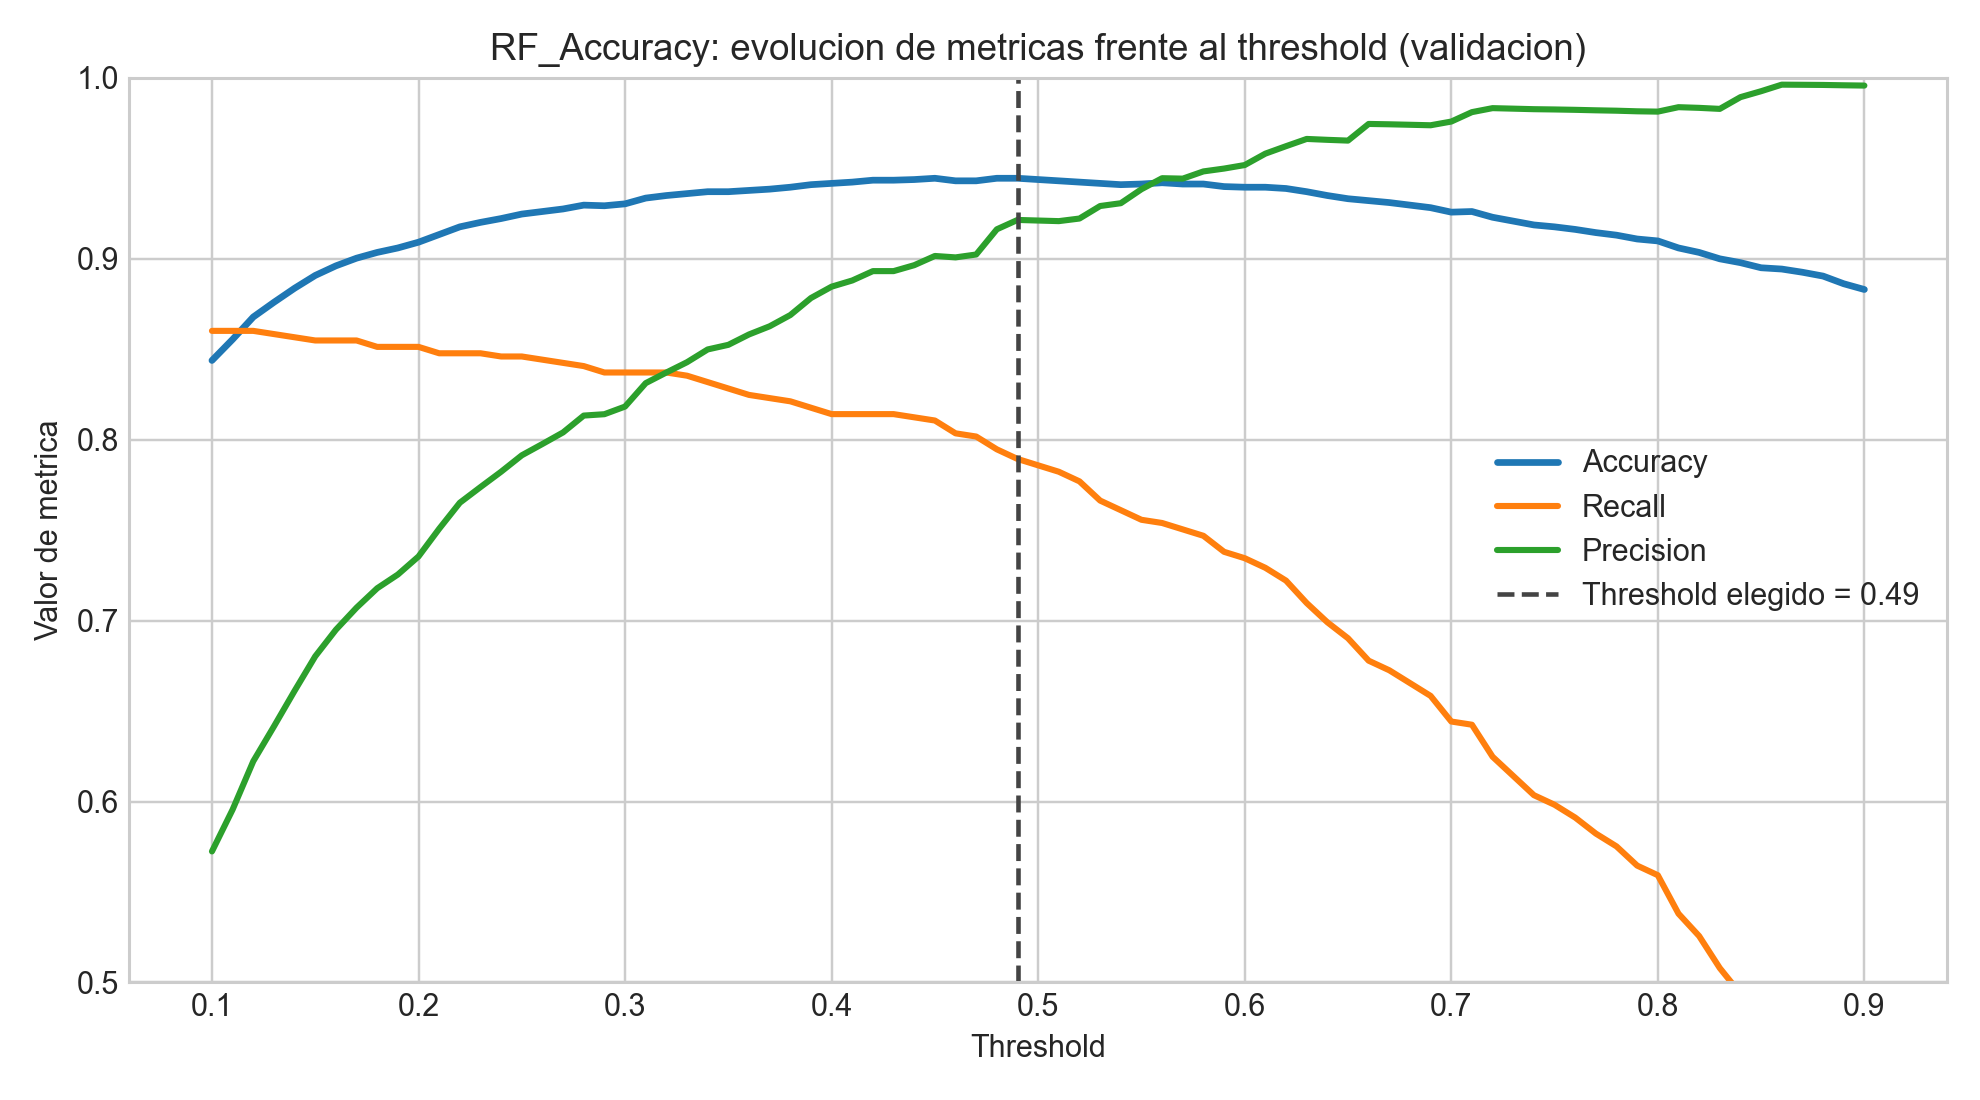
\includegraphics[width=0.9\textwidth]{figures/fase3_threshold_tradeoff_accuracy.png}
\caption{RF\_Accuracy: evolución de Accuracy, Recall y Precisión frente al threshold en validación.}
\label{fig:threshold_accuracy}
\end{figure}

\begin{figure}[h]
\centering
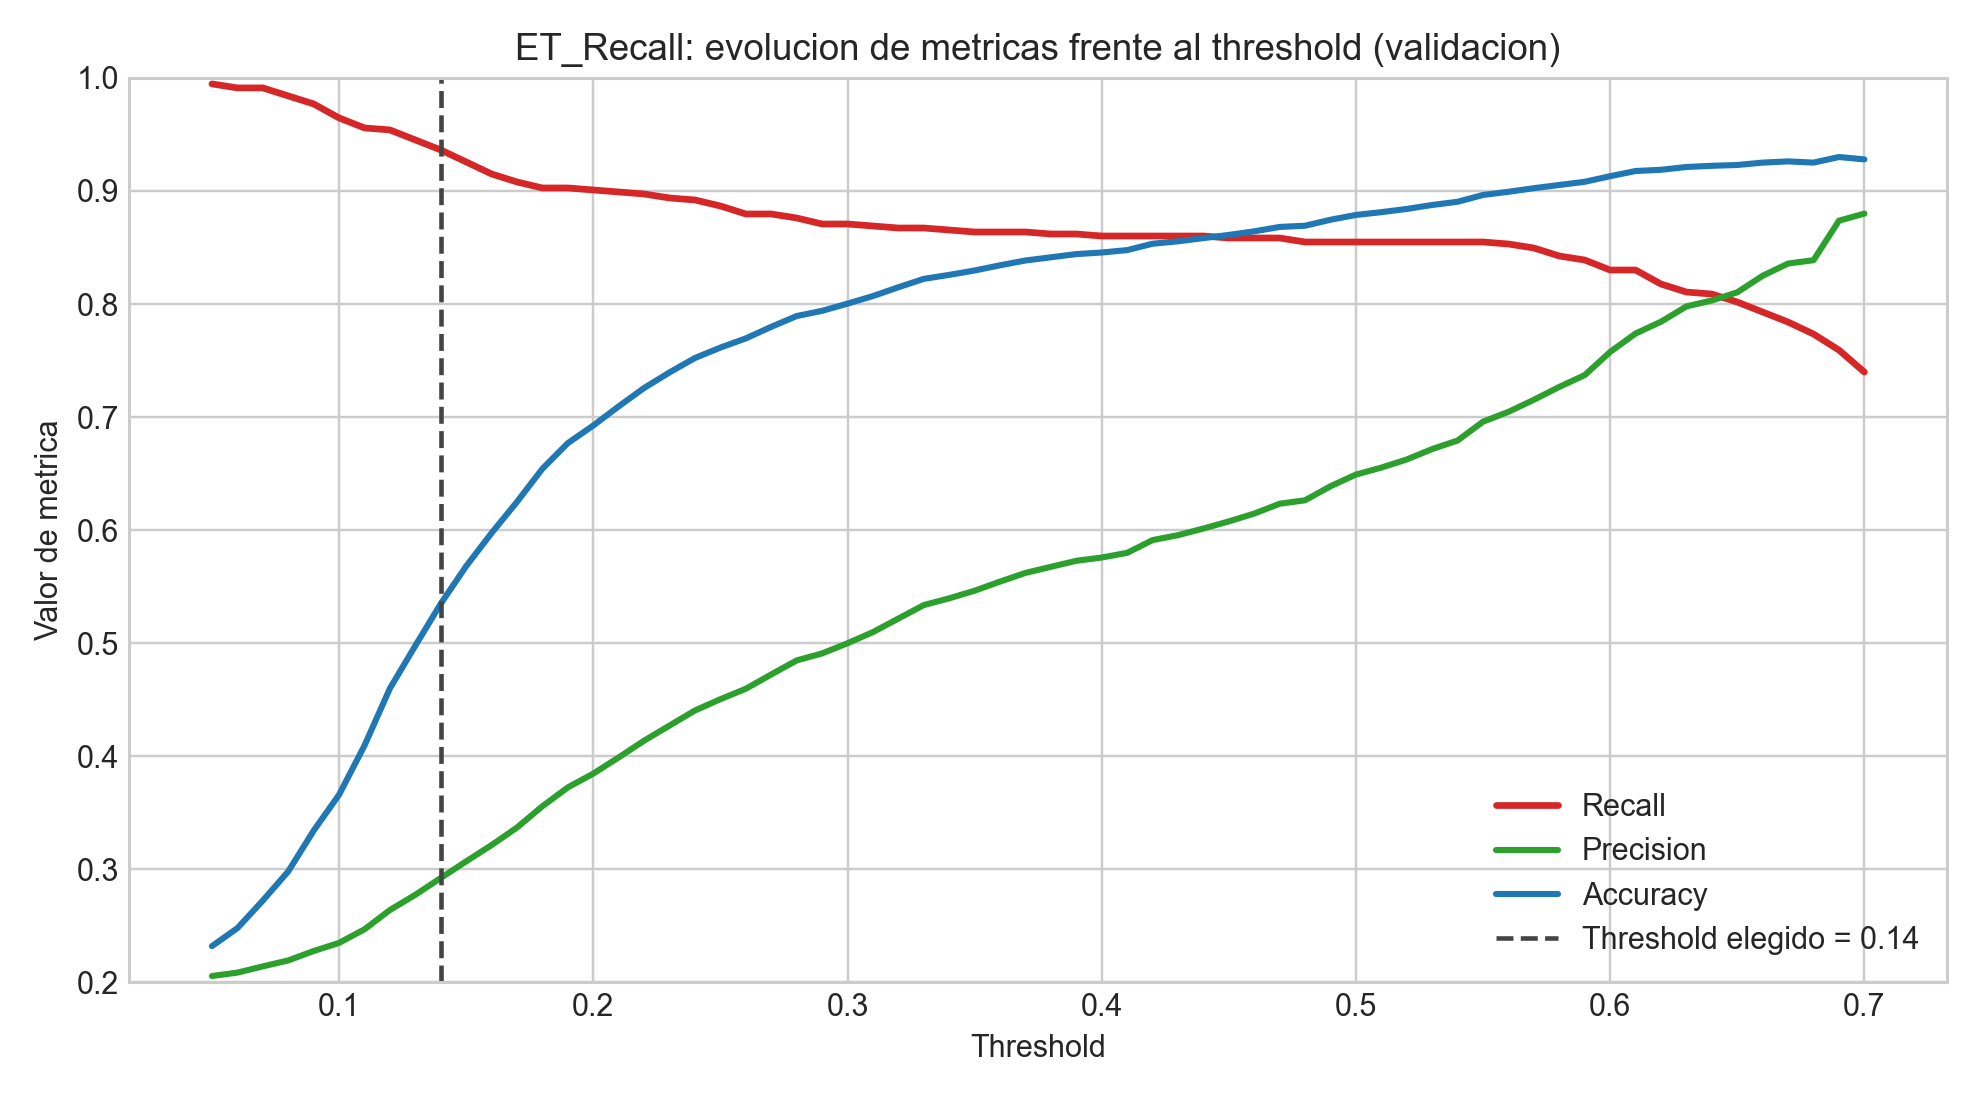
\includegraphics[width=0.9\textwidth]{figures/fase3_threshold_tradeoff_recall.png}
\caption{ET\_Recall: evolución de Recall, Precisión y Accuracy frente al threshold en validación.}
\label{fig:threshold_recall}
\end{figure}

\subsection{Sensibilidad de los guardrails para Recall}

El modelo ET\_Recall satisface los guardrails definidos:

\begin{itemize}
  \item \textbf{Precisión mínima:} 0.299 $>$ 0.25 \checkmark
  \item \textbf{PR-AUC mínimo:} 0.881 $>$ 0.80 \checkmark
\end{itemize}

Por tanto, ET es válido como modelo de alta cobertura, pero con mayor carga operativa.

\subsection{Síntesis operativa}

En términos de uso real, RF\_Accuracy es más eficiente cuando se prioriza precisión de campaña, mientras que ET\_Recall es útil como capa de exploración para no perder casos positivos.

\subsection{Recomendación}

Dado el contexto de retención de clientes:

\begin{enumerate}
  \item \textbf{Producción}: usar \textbf{RF\_Accuracy} como modelo principal por su mejor precisión global.
  \item \textbf{Análisis complementario}: usar \textbf{ET\_Recall} para ampliar cobertura y detectar casos potenciales no capturados por RF.
  \item \textbf{Monitoreo}: revisar periódicamente accuracy/recall para detectar deriva y ajustar threshold.
\end{enumerate}

En conclusión, \textbf{RF\_Accuracy} se selecciona como modelo principal y \textbf{ET\_Recall} se mantiene como apoyo para escenarios de cobertura máxima.

\section{Conclusiones}

En esta sección se sintetizan los hallazgos principales, las limitaciones del estudio y las conclusiones metodológicas y prácticas derivadas de la comparación entre los enfoques.


\appendix
\section{Apéndice}

Se incluirá aquí material auxiliar breve, como tablas resumidas, configuraciones relevantes o detalles complementarios que no convenga llevar al cuerpo principal del informe.


% Muestra todas las entradas del archivo .bib aunque no se citen en el texto.
\nocite{*}

\bibliographystyle{plainnat}
\bibliography{bibliography}

\end{document}
